\chapter{Proposta de Uso de Outliers no GeoGuide}
\label{chap:outliers}

Neste capítulo será abordado mais detalhadamente as características dos pontos que são considerados \textit{discrepantes (Outliers)}  em um determinado conjunto de dados e quais as influências que isso pode trazer para uma pesquisa. Além disso, vai ser falado do tratamento proposto para o GeoGuide e qual sua utilização. Também será detalhado o algoritmo escolhido e as motivações que levaram à essa escolha.

\section{Dados espaciais discrepantes}

Quando temas como a captura e análise de dados são tratados no cotidiano, o cenário atual se encontra numa situação única na história, já que nunca houve tanto volume de dados sendo gerado a todo segundo e das mais diversas formas e fontes. Caso seja aprofundado ainda mais nesse meio e focado em dados espaciais, será encontrado uma variedade de características específicas desse nicho e também problemas específicos os quais são buscadas solução.

Será destacado aqui 3 exemplos distintos de datasets que estão disponíveis atualmente na internet e são referentes a dados espaciais, cada um com sua particularidade:

\subsection{Táxis de Nova Iorque}

Desde de 2011 que as empresas de táxis de Nova Iorque, visando entender melhor seu funcionamento, conhecer mais sobre seu mercado e evitar as ocorrências de fraudes, investem em uma estrutura para coleta e armazenamento dos dados referentes a cada corrida de táxi que acontece na cidade. O resultado disso é que anualmente são armazenados e disponibilizados gigabytes de dados referentes a cada uma dessas corridas e que podem ser utilizados para análises de qualquer natureza e finalidade.

Entretanto, não é tão simples o processo de análise de volumes desse porte e antes mesmo dessa análise começar, vários fatores tem que ser levados em consideração, como, por exemplo, a estrutura desses dados e a confiabilidade dele. No caso desse dataset, falhas podem ocorrer nos equipamentos responsáveis pela coleta, no próprio gerenciamento e organização desses dados, pois esse processo necessita de intervenção humana e isso por si só é um fator de risco em qualquer análise.

Imagine que num determinado táxi em um certo dia e horário, todas as corridas tiveram o dado referente a distância percorrida pelo táxi com um valor negativo, o que fazer nessa situação? Ou então que a data início de uma corrida seja superior à data de término da mesma? Ou até sejam valores próximos, mas sua distância seja extremamente alta para esse tempo? Todos esses problemas podem acontecer nesse contexto e cada um deles devem ser tratados propriamente e com o devido cuidado. Esses tipos de problemas são os problemas no processo de \textit{limpeza dos dados} e é de uma importância crucial que eles sejam mitigados, pois nessas circustâncias as futuras análises estariam todas comprometidas com a presença de \textit{ruídos} que afetam diretamente uma boa análise.

\subsection{Hospedagens de Paris}

De maneira similar aos datasets sobre viagens de táxis, existem também grandes volumes de dados espaciais sobre hospedagens ao redor do mundo disponíveis na internet através da plataforma Airbnb\footnote{\it http://www.airbnb.com}, que é um serviço online para divulgações de hospedagens, com um diferencial, pois os lugares são divulgados por pessoas comuns e que, geralmente, vivem no local que querem divulgar.

Esses datasets podem ser utilizados para as mais diversas análises e com os mais diferentes propósitos. A sua estrutura consiste em dados espaciais (latitude e longitude) referente à hospedagem e os dados sobre a própria localidade em si, como por exemplo: o nome do anfitrião, o preço diário daquele local, a quantidade mínima de noites para poder alugar aquele lugar, a quantidade de dias que aquele imóvel está disponível no ano e etc.

Por exemplo, existe uma plataforma online que utilizou esses datasets para entender mais sobre esse mercado de hospedagens e se realmente, como proposto pela empresa Airbnb, esse novo mercado é uma alternativa às industrias de hotéis que existem pelo mundo. Quando analisado os dados e os volumes são agrupados pelas cidades ao redor do mundo, se percebe que esse novo mercado não é tão disruptível assim e que, na realidade, a maioria dos locais disponíveis para hospedagens são imóveis completos, gerando assim uma nova indústria mais moderna de hospedagens. Mais informações sobre essa pesquisa podem ser encontradas na plataforma disponível online no link \url{http://insideairbnb.com}.

Nesse tipo de dataset é possível utilizar técnicas e algoritmos de detecção de outliers para conseguir encontrar possíveis anomalias em regiões em que essa proposta de aluguel de residência não esteja de acordo com sua proposta inicial. Uma estrategia para isso é agrupar os pontos (sendo cada um uma residência para alugar) por regiões (nesse caso as cidades) e calcular quantas residências são propriedades da mesma pessoa. Com esse cruzamento de dados, poderia ser executado algum algoritmo de detecção de outlier e cada caso encontrado nessa abordagem vai indicar que existem pessoas que aproveitaram a ideia inicial do Airbnb para acabar construindo uma espécie de indústria alternativa de hospedagem.

\subsection{Restaurantes em Las Vegas}

Por fim, como mais um exemplo, existe outro conjunto de datasets espaciais referentes a restaurantes disponíveis em várias regiões pelo mundo. Esse conjunto é mantido pela empresa Yelp\footnote{\it https://www.yelp.com/} que oferece um serviço de pesquisa de restaurantes de forma personalizada que pode levar em consideração vários argumentos de acordo com sua necessidade, por exemplo: o local em que você queira encontrar os restaurantes próximos, o tipo de restaurante, a faixa de preço do seu interesse, enfim, uma porção de possibilidades para sua consulta.

Com essa estrutura é possível realizar diversas análises focadas em soluções específicas e que possam contribuir para contextos mais complexos. Essas possibilidades são tão frequentes que existe um desafio da própria empresa Yelp que convida estudantes de cursos superiores para submeterem propostas de análises desses conjuntos de dados voltadas para um tema específico e que acabem resolvendo problemas da própria empresa. As informações mais detalhadas desse desafio podem ser encontradas nesse site da Yelp \url{https://www.yelp.com/dataset/challenge}.

Incentivos como esse mostram o quão importante é o investimento nas áreas de análises de dados espaciais e o quanto ainda se pode aprimorar nessas análises para trazer informações mais úteis sobre os datasets e o que se pode fazer com esses determinados conjuntos de dados. Isso é uma das provas que essas análises podem ser tarefas complexas e que precisa-se de conhecimento mais qualificado para se conseguir melhores resultados.

\section{Outliers no GeoGuide}

Como dito anteriormente, o GeoGuide visa melhorar a experiência do analista frente à grandes montantes de dados espaciais que possam o deixar perdido durante sua análise, e isso, na maioria dos casos, prejudicará sua análise fazendo com que ele não leve em consideração informações que podem ser relevantes para sua pesquisa. Além disso, a existência de Outliers num dataset pode ser uma fonte de novas informações sobre aquele conjunto de dados. Por exemplo, em um conjunto de dados referente aos gastos do cartão de crédito de uma pessoa, caso tenha outliers, é um indicador muito forte de uma fraude nesse cartão, com isso, as empresas financeiras podem tomar medidas de segurança para evitar esses problemas.

No caso de datasets espaciais, as aplicações podem ser ainda maiores, pois além dos atributos referentes aos próprios pontos do conjunto, os próprios atributos referentes a localização do ponto (latitude e longitude) podem, por si só, caracterizar determinado ponto como um outlier. Dessa forma, a identificação desses pontos durante a análise do pesquisador pode trazer novas informações que estimule a criação de novas abordagens e decisões sobre aquele conjunto.

Sabendo disso, é possível aplicar essa detecção de outliers no GeoGuide enquanto o analista está no processo de descobrimento do dataset. Dessa forma, enquanto ele vai percorrendo pelo conjunto de dados e selecionando quais os pontos são de seu interesse, a ferramenta vai procurando, de forma assíncrona e implícita, pontos que podem ser outliers em relação aos pontos já previamente definidos como interessantes para o usuário e assim, de forma totalmente transparente e sem precisar de nenhuma nova ação do analista, novas informações sobre o dataset podem ser destacadas para quem está analisando e abrir um leque maior de opções e ideias sobre aquele conjunto de dados, ampliando sua análise mais facilmente e lhe mostrando o quê mais pode ser importante naquele ambiente.

\begin{figure*}[t]
	\centering
	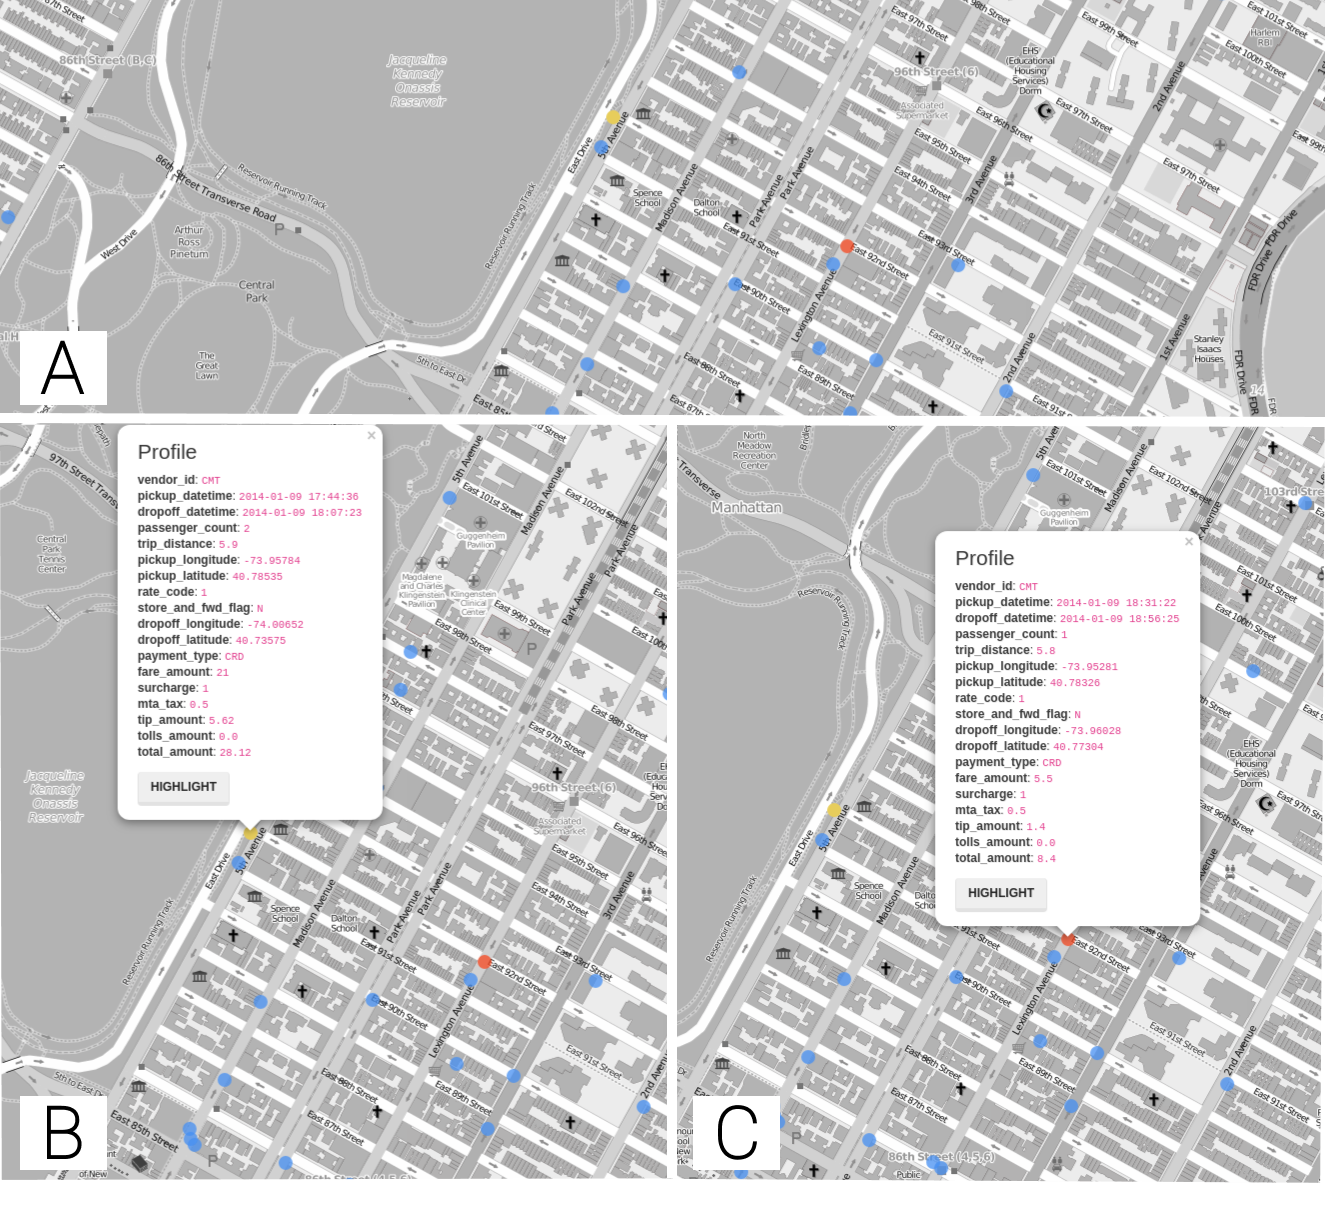
\includegraphics[width=\textwidth]{images/outliers-geoguide.png}
	\caption{Figura de um exemplo de uso de outliers no GeoGuide}
	\label{fig:outliers-geoguide}
	\vspace{-10pt}
\end{figure*}

A título de exemplo, pegando-se um dataset referente aos táxis de Nova Iorque e selecionando um conjunto de corridas de uma parte de Manhattan do mesmo dia e mesmo horário e com uma margem próxima de preço entre elas (na Figura \ref{fig:outliers-geoguide}.A o analista está explorando o dataset e seleciona um determinado ponto, no caso da imagem o ponto marcado em amarelo), pode-se buscar por pontos considerados outliers em relação ao seu preço com o conjunto e, com isso, detectar possíveis fraudes no serviço de táxi, caso esse ponto seja um outlier por um preço ``abaixo do normal'' ou então abuso de cobrança por parte do motorista se esse ponto for um outlier por um preço ``acima do normal''.

Na Figura \ref{fig:outliers-geoguide}.B o analista vê os atributos do ponto, marcado com a cor amarela, de sua escolha tais como distância (\textit{trip distance}) de $5,9km$ e preço de \$28,12  (\textit{total amount}) e um ponto considerado um outlier marcado pela cor laranja. Já na Figura \ref{fig:outliers-geoguide}.C é possível ver mais detalhes sobre o outlier e perceber que ele tem distância de $5,8km$ e o preço de \$8,4 doláres, sendo assim um outlier com um preço muito inferior ao padrão. Essa caraterística pode indicar uma viagem fraudosa e essa informação pode ser obtida de forma simples e interativa na plataforma. Sendo assim, de uma forma mais simples o analista tem condições de ir descobrindo novas particularidades que possam agregar muito ao seu conhecimento sobre aquele dataset.

Tomando como base essa situação, utilizar técnicas para detecção de outliers no GeoGuide traz a vantagem de que o analista, durante a exploração de um novo conjunto de dados, pode ir além na descoberta daquele dataset e encontrar rapidamente \textit{anomalias} que possam indicar que existe ``algo a mais'' nesses dados e isso reduz o tempo que ele gastaria se fosse explorar primeiro o dataset e depois ir atrás de pontos aberrantes, já que a própria ferramenta faria isso de forma paralela e só o notificaria quando surgisse algo que pudesse chamar sua atenção.

\section{Algoritmo}

O algoritmo proposto para ser utilizado nessa abordagem de detecção de outliers no GeoGuide \cite{omidvarTehrani2017} é o \textbf{LOF} \textit{(Local Outlier Factor)} \cite{Breunig:2000:LID:335191.335388}, pois ele tem as características que melhor se enquadra na abordagem com suas respectivas limitações. Uma importante propriedade desse algoritmo é que sua forma de considerar se um determinado ponto $p$ do conjunto $\mathcal{S}$ é um outlier leva em consideração não o conjunto completo, mas somente a relação do ponto $p$ com seus vizinhos. Isso torna o algoritmo LOF apropriado para conjuntos em que o que importa é o contexto de uma determinada região, e não todas caraterísticas do dataset.

\begin{algorithm}[!h]
	\DontPrintSemicolon
	\KwIn{Número de vizinhos $k$, conjunto de pontos $\mathcal{S}$}
	\KwOut{Vetor de fatores de densidade local $\mathcal{LOF}$}
	$\mathcal{LOF} \gets \emptyset$\;
	\ForEach{$p \in \mathcal{S}$}
	{
		$\mathcal{K}NNeighbors \gets \mathit{k\_distance}(\mathcal{S}, k)$\label{ln:k_distance}\;
		$lrd \gets \mathit{reach\_dist\_k}(\mathcal{K}NNeighbors, k)$\label{ln:reach_dist_k}\;

		\ForEach{$p \in \mathcal{K}NNeighbors$}
		{
			$templof[i] \gets sum(lrd[o \in \mathcal{N} (p)])(lrd[i])|\mathcal{N}(p)|$\;
			$\mathcal{LOF}.append(max(lof, templof))$\;
		}
	}
	$\mathcal{LOF} \gets top(\mathcal{LOF})$\;
	\Return{$\mathcal{LOF}$}\;  
	\caption{Cálculo dos fatores de discrepância local}
	\label{algo:lof}
\end{algorithm}

Sua função consiste na execução de um \textit{loop} que percorrerá todos os pontos do conjunto $\mathcal{S}$ em busca de calcular o seu grau de discrepância baseado nos seus vizinhos \cite{DBLP:conf:AlshawabkehJK10}. Primeiro ele calcula os $k$ vizinhos mais próximos do ponto $p$ e retorna uma matriz desses vizinhos com suas respectivas distâncias entre o ele e $p$ (linha \ref{ln:k_distance} do Algoritmo \ref{algo:lof}). Então, com essa matriz, ele calcula a densidade de acessibilidade desses vizinhos (linha \ref{ln:reach_dist_k} do Algoritmo \ref{algo:lof}) e entra num outro \textit{loop} para cada um dos $k$ vizinhos. Lá dentro ele processa as densidades desses vizinhos com o primeiro ponto $p$ e adiciona a maior densidade ao vetor $\mathcal{LOF}$ resultante. Por fim, ele retorna esses vetores ordenado de forma decrescente. 

Uma segunda particularidade importante desse algoritmo é que seu foco não é definir ``binariamente'' se um determinado ponto é um outlier ou não, mas sim ``o quão'' outlier é esse ponto em relação aos seus vizinhos e o contexto daquela região. Isso faz com que ele consiga detectar pontos com nuances de um outlier de uma forma que outros algoritmos não conseguem, pois essas nuances não cruzariam o limite de definição de outlier, mas já poderia destacar aquele ponto como um possível foco de observação para conhecer melhor o dataset.

Além disso, esse fator não binário é melhor de ser processado pelo GeoGuide por ser um valor númerico, podendo ser até considerado como um novo atributo de cada ponto do conjunto. Esse atributo pode ser incorporado mais facilmente no processamento de orientação da ferramenta e as nuances de discrepância entre os pontos será refletida nas recomendações do GeoGuide. Se esse fator fosse binário, o GeoGuide precisaria planejar qual o peso que tal fator teria para o procedimento de sugestões de novos pontos.